\documentclass[../main.tex]
		
		\begin{document}
			\section{Eulerian trails and circuits}
	\begin{description}
		\item[Task:] Look at trails and circuits that traverse every edge of a graph. Derive criteria when such trails and circuits exist.
		\item[Definition:] An \underline{Eulerian trail} in a graph is a trail that traverses every edge of that graph. In other words, an Eulerian trail is a walk that traverses every edge of the graph exactly once. \\
		Trail $\Rightarrow$ an edge is traversed at most once. \\
		Eulerian $\Rightarrow$ every edge is traversed.
		\item[Definition:] An \underline{Eulerian circuit} is a graph is a circuit that traverses every edge of the graph.
		\item[Origin of the terminology:] Eurlerian comes from the swiss mathematician Leonhard Euler (1707-1783) who solved the problem of the seven bridges of k\"onigsbey/kaliningrad (Then Prussia, now Russia) over the river Prugal in 1736. His negative sollution is considered the beginning of graph theory as a subfield of mathematics. We will rederive Euler's results shortly. Google to see the configuration of the bridges on the river Prugel.
		\item[Examples:]
		\begin{enumerate}
			\item[]
			\item $abc$ is an Eulerian trail and an Eulerian circuit. The triangle is $k_3$.
			\begin{figure}[h!]
				\centering
				\begin{tikzpicture}
				\draw (0,0) node[above]{A} -- (-1,-2) node [left]{B} -- (2, -2) node[right]{C} -- (0, 0);
				\end{tikzpicture}
			\end{figure}
			\item Consider $k_5$, the complete graph with 5 vertices. \\
			$eabecdbcade$ is an Eulerian circuit.
			\begin{figure}[h!]
				\centering
				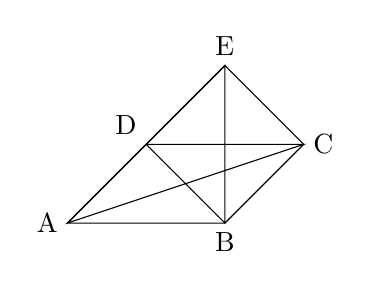
\begin{tikzpicture}
				\coordinate (E) at (0, 0);
				\coordinate (C) at (1, -1);
				\coordinate (D) at (-1, -1);
				\coordinate (B) at (0, -2);
				\coordinate (A) at (-2, -2);
				
				\draw (A) node[left]{A} -- (E) node[above]{E} -- (C) node[right]{C} -- (B) node[below]{B} -- (A);
				\draw (D) node[above left]{D} -- (B) -- (E) -- (A) -- (C) -- (D);
				\end{tikzpicture}
			\end{figure}
		\end{enumerate}
		In both cases, the degree of the vertices is even for all vertices. We'll see this property is important and derive other necessary and sufficient conditions for the existence of Eulerian trails and circuits.
		\item[Theorem:] Let $(V, E)$ be a graph, and let $v_0 v_1 \dots v_m$ be a trail in $(V, E)$. Let $v \in V$ be a vertex, then the number of edges of the trail incident to $v$ is even except when the trail is not closed and the trail starts and finishes at $v$, in which case the number of edges of the trail incident to the vertex $v$ is odd.
		\item[Proof:] Note that 0 is an even integer as 0 = 2 $\times$ 0.
		\begin{description}
			\item[Case 1:] $v \neq v_0 \land v \neq v_m$. If the trail does not pass through $v$, the number of dges incident to $v$ belonging to the trail is 0, which is even. \\
			If the trail passes through $v$, then edges of the trail incident to $v$ are of the form $v{i-1} v_i$ and $v_i v_{i+1}$ with $v = v_i$ and $0 < i < m$. Therefore, the number of edges of the trail incident to $v$ equals twice the number of integers $i$ among $1, 2, \dots, m-1 (0 < i < m)$ s.t. $v= v_i \Rightarrow$ the number of even.
			\item[Case 2:] $v = v_0$ and the trail is not closed, \textbf{i.e.} $v_m \neq v_0$. The edges incident to $v$ are $v_0 v_1$ along with $v_{i-1} v_i$ and $v_i v_{i+1}$ whenever $v=v_i$, hence 1+2. $\#$(instances when $v=v_i$), which is odd.
			\item[Case 3:] $v=v_m$ and the trail is not closed, \textbf{i.e.} $v_m \neq v_0$. Repeat the argument in case 2 with $v_{m-1} v_m$ replacing $v_0 v_1$ to get that the number of edges incident to $v$ is odd.
			\item[Case 4:] The trail is closed and $v = v_0 = v_m$. The edges incident to $v$ are $v_0 v_1, v_{m-1} v_m$ as well as $v_{i-1} v_i$ and $v_i v_{i+1}$ for each $i$ s.t. $v=v_i \Rightarrow$ once again, the number of edges incident to $v$ is even.
			\item[qed]
		\end{description}
		\item[Corollary 1:] Let $v$ be a vertex of the graph. Given any circuit in the graph, the number of edges incident to $v$ traversed by that circuit is even.
		\item[Proof:] Apply the theorem to $v_0 v_1 \dots v_m$ s.t. $v_0 = v_m$. We deduce that the number of edges incident to $v$ is even.
		\item[Corollary 2:] If a graph admits an Eulerian circuit, then the degree of every vertex of that graph must be even.
		\item[Proof:] Let $(V, E)$ be the graph. $\forall v \in V$, the number of edges of any Eulerian circuit incident to $v$ is even by the previous corollary. Since an Eulerian circuit by definition traverses every edge of the graph, every edge incident to $v$ is an edge of the Eulerian circuit $\Rightarrow$ deg $v$ is even $\forall v \in V$ (\textbf{NB:} def $v$ could be zero if $v$ is an isolated vertex).
		\item[Example:] By the previous corollary, $k_4$, the complete graph on four vertices, cannot have an Eulerian circuit since $\forall v$ in $k_4$, def $v = 3$ ($k_4$ is 3-regular as we bserved in a previous lecture).
		\item[Corollary 3:] If a graph admits an Eulerian trail that is not a circuit, then the degrees of exactly two vertices of the graph must be odd, and the degrees of the remaining vertices must be even. The vertices with odd degrees are exactly the initial and final vertices of the Eulerian trail.
		\item[Proof:] By the theorem, the initial and final vertices of the Eulerian trail have odd degree, whereas all vertices in between have even degrees.
		\item[qed] 
	\end{description}
	Next, prove the \underline{converse} of corollary 2: A non=trivial connected graph has an Eulerian circuit if the deree of each of its vertices is even. The proof is carried out in a series of lemmas:
	\begin{description}
		\item[Lemma A:] If the degree of each vertex is even, the $\exists$ a circuit.
		\item[Lemma B:] If the degree of each vertex is even, if $\exists$ circuit, and if $\exists$ edges not in the circuit incident to a vertex in the circuit, we can construct another circuit.
		\item[Lemma C:] If we have two circuits with at least one vertex in common, we can combine them.
		\item[Lemma D:] A criterion for when a trail in Eulerian in a connected graph.
		\item ~\\
		\item[Lemma A:] Let $vw$ be an edge of a graph in which the degree of every vertex is even, the $\exists$ circuit of the graph that traverses the edge $vw$.
		\item[Proof:] We construct the circuit starting with the edge $vw$. Let $v_0 = v$ and $v_1 = w$. Let $v_0 v_1 \dots v_k$ be any trail of length $k \geq 1$ traversing the edge $vw$. Suppose $v_k \neq v = v_0$. As we proved in the previous theorem, since $v_k$ is an endpoint of a non-closed trail, then the number of edges of the trail incident to $v_k$ is odd, but deg $v_k$ is even $\Rightarrow \exists$ edge of the graph incident to $v_k$ that is not traversed by the trail $v_0 v_1 \dots v_k$. Let $v_k v_{k+1}$ be this edge, then $v_0 v_1 \dots v_k v_{k+1}$ is a trail of length $k+1$ that starts at $v$ and traverses $vw$. Since every edge of the graph is traversed at most once by a trail, the length of any trail in the graph cannot be greater than the number of edges of the graph $\#(E)$. We have shown above that if our trail is not closed, then it can be extended. By successive extensions, we will eventually have constructed a trail that cannot be extended (in at most $\#(E)-1$ steps). Therefore, that trail must be closed. As the edge $vw$ is traversed, this trail in nontrivial $\Rightarrow$ it is a circuit.
		\item[qed]
		\item[Lemma B:] Let $(V, E)$ be a connected graph s.t. $\forall v \in V$, deg $v$ is even, and let some circuit $v_0 v_1 \dots v_{m-1} v_0$, then $\exists$ another circuit in $(V, E)$ passing through $v_i$ that does not traverse any edge traversed by $v_0 v_1 \dots v_{m-1} v_0$.
		\item[Proof:] Let $E'$ be the set of edges not traversed by $v_0 v_1 \dots v_{m-1} v_0$. $(V, E'$ is a subgraph of $(V, E). \forall v \in V, \#$ of edges of $v_0 v_1 \dots v_{m-1} v_0$ incident to $v = d(v) - d'(v)$, where $d(v) =$ def$(v) = \#$ of edges in $(V, E)$ incident to $v$ and $d'(v) = \#$ of edges in $(V, E')$ incident to $v$. By Corollary 1, $d(v) - d'(v)$ is even, but by assumption $d(v) =$ deg $v$ is even $\Rightarrow d'(v)$ is even $\Rightarrow$ the degree of every vertex in the subgraph $(V, E')$ is even. Now consider the vertex $v_i$ in the statement of Lemme B. Some but not all edges incident to $v_i$ are traversed by $v_0 v_1 \dots v_{m-1} v_0 \Rightarrow d'(v_i) > 0$, \textbf{i.e.} at least one edge incident to $v_i$ is in the subgraph $(V, E')$. We are now \underline{exactly} in the scenario described by Lemma A $\Rightarrow$ by Lemma A, $\exists$ circuit in $(V, E')$   passing through $v_i$. This circuit is also a circuit in $(V, E)$ as $(V, E')$ is a subgraph of $(V, E)$, and since all of its edges are in $E'$, this other circuit does not traverse any edge traversed by $v_0 v_1 \dots v_{m-1} v_0$
		\item[qed]
		\item[Lemma C:] Suppose that a graph contains a circuit of length $m$ and a circuit of length $n$. Suppose also that no edges of the graph is traversed by both circuits, and that at least one vertex of the graph is common to both circuits, then the graph contains a circuit of length $m+n$.
		\item[Proof:] Let $v$ be a vertex of the graph that is common to both circuits. We assume both circuits start and finish at the vertex $v$. Let the first circuit be $vv_1 \dots v_{m-1} v$, and let the second circuit be $vw_1 w_2 \dots w_{n-1} v$. We concatenate the two circuits obtaining a circuit $vv_1 \dots v_{m-1}vw_1w_2 \dots w_{n-1}w$ of length $m+n$
		\item[qed]
		\item[Lemma D:] Let $(V, E)$ be a connected graph, and let some trail in this graph be given. Suppose that no vertex of the graph has the property that not all the edges of the graph incident to that vertex are traversed by the trail. Then the given trail is an Eulerian trail.
		\item[Proof:] Let $v_1$ be the set of vertices through which the trail passes, and let $v_2$ be the set of vertices through which the trail does not pass. $v=v_1 \cup v_2 \land v_1 \cap v_2 = \emptyset$. The conclusion of Lemma D amounts to showing $v_2 = \emptyset. \forall u \in v_1, u$ is incident to at least one edge traversed by the trail. $\Rightarrow$ all edges incident to the vertices in $v_1$ are traversed by the trail, but then every vertex in $v$ adjacent to a vertex in $v_1$ must belong to $v_1 \Rightarrow$ no edge can join a vertex in $v_1$ to a vertex in $v_2$. If $v_2 \neq \emptyset$, then $\exists w \in v_2$, but then $w$ cannot be joined by a path to any vertex in $v_1 \Rightarrow v_1 \land v_2$ are in different connected components of the graph $\Rightarrow \Leftarrow$ since the graph is connected $\Rightarrow$ it has only one connected component. Therefore, $v_2 = \emptyset$.
		\item[qed]
	\end{description}
	Finally, we can prove Euler's theorem:
	\begin{description}
		\item[Theorem] A non-trivial connected graph contains an Eulerian circuit if the degree of every vertex of the graph is even.
		\item[Proof:] Let $(V, E)$ be a non-trivial connected graph s.t. $\forall v \in V$, deg $v$ is even. By Lemma A, $(V, E)$ contains at least one circuit. It therefore contains a circuit of maximal length (\textbf{i.e.} at least as long as any other circuit in the graph). We seek to prove that this circuit of maximal length is indeed Eulerian. \\
		If the graph contains some vertex $v$ s.t. some but not all of the edges of the graph incident to $v$ are traversed by the circuit of maximal length, and $v$ is a vertex on the circuit of maximal length, then by Lemma B $\exists$ a second circuit in $(V, E)$ passing through $v$, which would not traverse any edge traversed by the circuit of maximal length. By Lemma C, however, we can concatenate the two circuits, obtaining a circuit of length strictly greater than the length of the circuit of maximal length $\Rightarrow \Leftarrow$ we conclude no vertex that belongs to the circuit of maximal length has the property that not all edges incident to it are traversed by the circuit of maximal length. Since $(V, E)$ is connected, by Lemma D, the circuit of maximal length must be Eulerian.
		\item[qed]
	\end{description}
	Corollary 2 along with this theorem together gives us:
	\begin{description}
		\item[Theorem:] A non-trivial connected graph has an Eulerian circuit $\Leftrightarrow$ the degree of each of its vertices is even.
		\item[Corollary:] Suppose a connected graph has exactly two vertices whose degree is odd. $\exists$ an Eulerian trail in the graph joining the two vertices with odd degrees.
		\item[Proof:] We reduce this case to the previous one by embedding the graph $(V, E)$ with vertices $v, w$ that have odd degree into a graph $(V', E')$ s.t. $v' = v \cup \{u\}$ for $u \notin V$ and $E' = E \cup \{uv, uw\}$. $(V, E)$ is a subgraph of $(V' E')$ and $(V', E')$ is connected and each one of its vertices has even degree by construction. By the theorem we just proved, $(V', E')$ has an Eulerian circuit. We reorder the vertices so that the final two edges are the two added edges $wu$ and $uv$. We now delete the edges $wu$ and $uv$ to obtain an Eulerian trail in the original graph $(V, E)$ from $v$ to $w$.
		\item[qed]
	\end{description}
	

\end{document}